\chapter{Implementation}

	In order to achieve the goals set in this project, two separate pieces of 
	software and one piece of hardware were written. The software programs are 
	two different implementations of a reference shader. The first of these was 
	written in GLSL for traditional graphics hardware (in our case it was 
	tested on a GeForce GTX 1060M), and the second is written in an assembly 
	language we designed for the Sphere Tracing processor. Both of these 
	shaders are described in section \ref{implshader}. The hardware is 
	comprised of a multi-core programmable parallel processing unit designed 
	for the Sphere Tracing algorithm, detailed in section \ref{implproc}. In 
	addition to these, a simple assembler was written for the assembly language
	used for the GPU.

	\section{Reference Shader} \label{implshader}

		The core of the Sphere Tracer is a simple while-loop. It calculates
		distance to the closest object in the scene by sampling the distance
		field and comparing its value at the current location to a predefined
		epsilon. If the value of the distance field is smaller, the ray has hit
		an object; the corresponding pixel's color is calculated and the loop
		is terminated, unless the material of the object in question is defined
		as being reflective.

		\subsection{GLSL Based}

			The shader which is made to run on conventional graphics hardware
			was made in the high-level shading language GLSL (short for OpenGL
			Shading Language). It runs the program for each pixel the shader is
			rendered on, using the screen-coordinates as input.

			Beyond the actual sphere tracing loop the direction of the ray is
			calculated using a camera direction vector and offsetting it by the
			current pixel's screen coordinates, placed orthogonally along the
			vector.  The distance of this placement defines the field of view
			of the camera. This needs to be done for each pixel being rendered.

			The final color of a pixel is based on the material ID assigned to
			the first object that the ray intersects. The color can then be
			either calculated by a material formula or be derived from a
			texture lookup. True 3D materials can be done by texturing but this
			generally needs a large data set and thus a formula is mostly
			preferred where three dimensional materials are employed. 2D
			texturing can be done by projecting points from a flat image onto a
			simple geometric shape  which is more or less enveloping the object
			in question. This is called texture-mapping and commonly uses
			simple shapes like planes, cubes, spheres and cylinders. 

			%FLOWCHART

		\subsection{Orthogonal culling}

			The most demanding parts of sphere tracing are that the distance to
			a lot of objects has to be calculated once for every march step.
			The number of steps taken depends on the scene but they can reach
			over a hundred. One way to increase the performance is to reduce
			the number of objects that the distance has to be calculated to,
			without reducing the actual number of objects in the scene. To do
			this the GPU needs to know which object a ray can't possibly hit,
			traditionally the CPU will tell the GPU which objects are in the
			field of view (Frustum culling) but we can't do that because of
			GLSL limitations. Even if we could use frustum culling it would
			probably not be enough, each ray should only care for the objects
			that it might hit, not all objects in the field of view.  An
			implementation of a method we call Orthogonal Culling was
			implemented.

			Orthogonal projection works by going through all the objects in the 
			scene for ray and calculating wheather the ray can hit the object
			or not. 

			To calculate whether the ray will hit a sphere or not orthogonal
			projection can be used. By projecting the center of the sphere onto
			the directional line of the ray, its closest point to the line is
			known.  Then the distance between the line and the sphere can be
			calculated using the radius, if the distance is less than zero the
			sphere will be hit by the ray. If the distance is larger than zero
			the ray can't possibly hit that sphere. This way the number of
			objects that the distance has to be calculated to is decreased.

		\subsection{Bounding spheres}
			
			Another way decrease the number of distance calculations that has
			to be performed in each march step is to enclose several objects in
			a march sphere. When the distance field is evaluated only the
			bounding sphere will be considered and none of the objects enclsed
			by it. If the bounding sphere is hit by the ray, it will be removed
			and all the contained objects will be introduced to the distance
			field. 

			In practice this was made by calculating the centrum of the
			objects, by adding together their position vectors and scale by the
			inverse of the number of objects, this point is the position of the
			bounding sphere. The radius of the sphere is simply the distance to
			the object that is the farthest from the center of the sphere plus
			it's "max radius", that is, for a cube with a side of length 2, the
			square root of 3. The way our bounding spheres was set up had some
			flaws, such as if huge objects are placed near origin of the
			bounding sphere it will only be partially rendered.

			%picture of example bounding sphere

		\subsection{GPU Assembler Based}

			In the assembler version that runs on our own hardware there is
			initially a single thread. This thread will create one new thread
			for each pixel on the screen, and this thread will calculate what 
			color the pixel should have and then terminate. This differs from 
			the shader version that simply runs the GLSL-code for each pixel
			in parallell at the graphics cards many cores.

	\section{Processor Unit} \label{implproc}

		The properties of the ray marching algorithm as described in chapter
		\ref{spheretracing} led to the decision of designing a GPU architecture
		that does not utilize multi-ALU SIMD with lockstepping to the same
		extent as traditional graphics processors. Instead, a solution with
		slightly simpler independent cores was decided upon. This is similar to
		reasoning employed by \cite{Woop2005} for a Ray Tracing hardware
		design.

		The hardware described in this section was written in \clash. \clash is
		based on the functional programming language Haskell and is therefore a
		functional hardware description language, or FHDL. One thing that
		\clash offered was the command-line repl that allowed us to quickly
		write and test new modules on a higher conceptual level rather than
		simulating the Verilog code on a bit level.

		\subsection{Architecture}

			The GPU is designed to be able to handle a form of threading
			natively, where all computations are performed by a thread running
			on some hardware core. A thread in this context is very
			light-weight: only an instruction pointer along with some mutable
			registers are stored.

			All threads that are not running are placed in a storage structure
			that is globally accessable to all cores, and threads are then
			dispatched to cores as the cores become available for execution.
			The cores are also able to spawn new threads by sending their data
			to the global storage, or terminate threads either by simply
			dropping them or by sending them to the frame buffer, where some of
			the registers will be used to determine the color of some pixel on
			the screen.

			Each core consists of instruction and data memories, some control 
			logic for execution order and a DFU. The data and instruction 
			memories are immutable and mirrored across all cores in their 
			entirety. The control logic is responsible for feeding the DFU with
			instructions and data, as well as updating the thread registers 
			when a new thread is attached, sending thread registers to the 
			global thread storage when new threads are spawned and and 
			requesting a new thread whenever the previously executing one 
			terminates.
			
			The DFU contains a stack which all arithmetic instructions operate
			on, as well as an ALU for carrying out calculations. It also keeps
			track of all the thread registers and updates them when such
			instructions are issued. The DFU contains very little extra control
			logic and is only able to receive and execute instructions, it does
			not keep track of any instruction pointers or when threads are
			attached or dropped, this is instead handled by the core control
			logic.

		\subsection{Instruction Set}

			A representation for distance functions was also designed. It is
			implemented as a reverse polish notation inspired stack based 
			instruction set.

			There are a total of four instruction types with different
			instruction encodings, their layout in memory is shown in figure
			\ref{encodingfig}, and the type of instructions are:

			\begin{description}
				\item[C-type] instructions are for control flow, that is, 
					instructions that affect the global queue or frame buffer or
					terminate the current thread. C-type instructions can be 
					conditionally executed, based on the condition encoded in
					the two highest bits in the opcode. 

				\item[D-type] instructions, which encode arithmetic- and vector
					instructions on the stack. These operate only on the
					internal stack in the core and not on any of the other
					registers. They can take up to six arguments and return up
					to three return values. D-type instructions can be split up
					in chunks using the \texttt{next} instruction, where the
					last computed result will be accumulated using the minimum
					automatically by the core.  This is useful for encoding
					distance functions.

				\item[V-type] instructions deal with memory accesses. The
					\texttt{p} bit encodes whether this access is for pack
					(mutable) or read-only memory.

				\item[R-type] instructions load wide immediate values into the
					DFU. They are currently only used for assigning distance
					function IDs.
			\end{description}

		\subsection{Execution Model}

			The processor contains a global storage structure that is shared
			among all cores, onto which all threads that are ready for
			execution wait until a core is ready to start executing them.

			\begin{figure}[H]
				\centering
				\caption{ XQBGPPPU Data flow diagram }
				\includegraphics[width=0.75\linewidth]{figure/dots/GPU-schematic.pdf} 
				\vspace{-4pt}
			\end{figure}
	
			Each shader thread has 16 mutable registers that are automatically
			loaded into the core when execution starts. These registers are
			also saved when execution pauses and they are also copied whenever
			a thread spawns a new child. The instruction \texttt{setval} can be
			used to change the value of a register, and the instruction
			\texttt{pack} reads the value of a register.

			All calculations are performed with intermediate values stored on a
			stack, with the ability to move any values between the stack and
			any of the registers using the \texttt{setval} and \texttt{pack}
			instructions.

			There are three main instructions for control flow: \texttt{pushq},
			\texttt{pushf}, and \texttt{drop}. Threads can spawn new threads at
			any time using the instruction \texttt{pushq}: this will cause the
			core to make a copy of all of the registers and push it onto the
			global queue, where another (or the same) core may later access
			them and start executing from the instruction pointer register
			(\texttt{r0}).

			Threads can also terminate execution in two ways. Executing the
			instruction \texttt{drop} will terminate the thread and discard all
			registers. Executing \texttt{pushf} will terminate the thread and
			discard all values except the pixel pointer (\texttt{r1}) and color
			register (\texttt{r2}), which will be sent to the frame buffer in
			order to be displayed on the screen.

			This set of instructions for control flow might initially seem to
			be neither useful nor easy to implement but they are powerful
			enough to implement for all branching that is needed in our ray
			marchers efficiently while being restrictive enough to make
			instruction memory accesses very predictable.

			In addition to this, each core can accelerate finding the minimum 
			distance for a set of distance functions using a built-in 
			accumulator, together with the instructions \texttt{next} and 
			\texttt{accum}. Because of this, distance functions can be written
			without any regard for how the shader that called them works, and
			this very common operation is automated, reducing the size of each
			distance function slightly.

		\subsection{Square Roots}

			Calculating distances is an integral part of the algorithm, so a
			good square root implementation was considered important for
			achieving good performance. Several different approaches for this
			were considered.

			Firstly, using an iterative method like Goldschmidt's or the
			babylonian method was considered. These require an initial starting
			value, which is usually generated using a look-up table. We tested
			a different and very fast method for generating an initial rough
			guess of the square root of any number without the need for a
			look-up table. A 16-bit version of this circuit is shown in figure
			\ref{orsqrt}, and an improved but slightly more expensive version
			is showed in figure \ref{orsqrt2}.  The basic working principle is
			based on the fact that the square root of a number har roughly half
			as many digits as the original number. In the version with slightly
			improved accuracy the placement of the extra wires is based on the
			bit pattern of $\sqrt{2}$.

			\begin{figure}
				\centering
				\caption{A simple square root approximator}
				\label{orsqrt}
				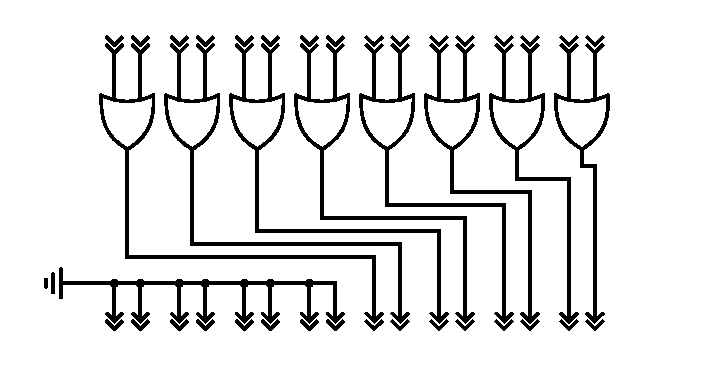
\includegraphics[width=0.75\linewidth]{figure/pdf/simpleOr.pdf} 
			\end{figure}

			\begin{figure}
				\centering
				\caption{Simple square root approximator with minor improvement.
					This version includes an extra layer of or-gates with a 
					shift of 4. Adding more layers with shifts of 6, 10, 14, 26
					etc increases accuracy further, although returns are 
					diminishing quickly.}
				\label{orsqrt2}
				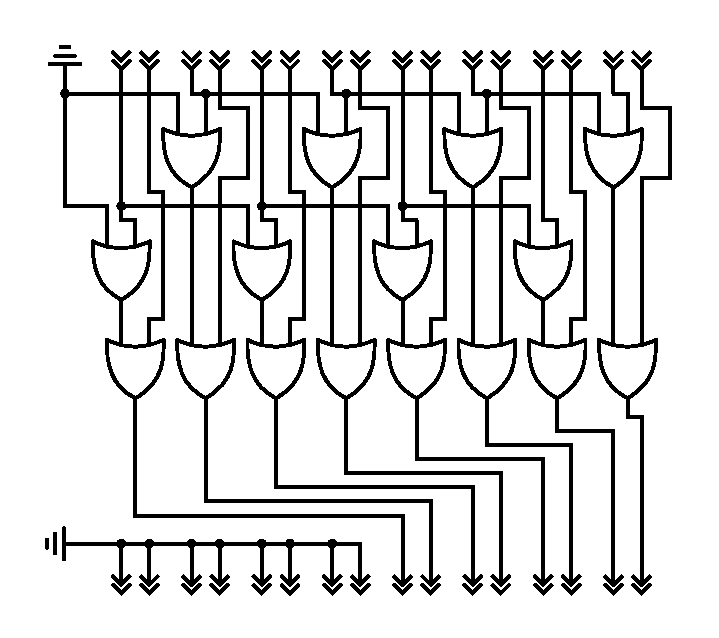
\includegraphics[width=0.75\linewidth]{figure/pdf/sqrt2Or.pdf} 
			\end{figure}

			In order to improve the accuracy of this method another design was
			considered in which the input was both rounded up and down to
			values where the simple square root approximator was very accurate
			and the result was then linearly interpolated between these roots.
			This linear interpolation requires only a multiplication and a
			couple of additions, but choosing upper and lower seed values is a
			more complex problem. Choosing the two geometrically closest powers
			of two was tested because the or-gate square root circuit is very
			accurate for powers of two, but this is not the only possible
			choice.

			\begin{table}
				\centering
				\caption{A \texttt{C} implementation of the shifting nth root 
					algorithm}
				\label{sqrtc}
				\begin{tabular}{c}
				\begin{lstlisting}
int isqrt(int num) {
    int res = 0;
    int bit = 1 << 30;

    while(bit != 0) {
        if(num >= res + bit) {
            num -= res + bit;
            res = (res >> 1) + bit;
        } else res >>= 1;
        bit >>= 2;
    }
    return res;
}
				\end{lstlisting}
				\end{tabular}
			\end{table}

			\begin{table}
				\centering
				\caption{A \texttt{C} implementation of the shifting nth root 
					algorithm}
				\label{sqrtcopt}
				\begin{tabular}{c}
				\begin{lstlisting}
int isqrt(int num) {
    int res = 0;
    int bit = 1 << 30;

    while(bit != 0) {
    	int tmp = num - (res | bit);
    	res >>= 1;
        if(tmp >= 0) {
            num = tmp;
            res |= bit;
        }
        bit >>= 2;
    }
    return res;
}
				\end{lstlisting}
				\end{tabular}
			\end{table}

			Another algorithm for calculating square roots is the
			\emph{Shifting nth root algorithm}, also known as \emph{Dijkstras
			square root algorithm}, which calculates the square root one digit
			at a time. A \texttt{c} implementation of this algorithm is shown
			in figure \ref{sqrtc}. Initially, this algorithm does not seem like
			a good canditate for a high performance hardware implementation,
			but several important optimizations are possible when unrolling it
			combinatorially. Most of the additions can be reduced to bitwise
			logic operations already when computing it in software, as shown in
			figure \ref{sqrtcopt}. In a combinatorial hardware implementation,
			these bitwise operations can be removed entirely by simply moving
			wires around, yeilding a logic cost of 0. The only remaining
			operations is therefore the subtraction on line 6, and the
			conditional assignments of \texttt{num} and \texttt{res} on lines 9
			and 10. The cost of the subtraction can be significantly reduced
			because \texttt{res} approximates the result one bit every step,
			meaning most bits are zeroed at any given iteration. On average,
			only 25\% of this subtraction is needed. This turned out to result
			in a design very similar to the PARSQRT implementation by
			\cite{japaneseSQRT}.
